% Created 2020-04-27 Mon 12:38
% Intended LaTeX compiler: pdflatex
\documentclass[11pt]{article}
\usepackage[utf8]{inputenc}
\usepackage[T1]{fontenc}
\usepackage{graphicx}
\usepackage{grffile}
\usepackage{longtable}
\usepackage{wrapfig}
\usepackage{rotating}
\usepackage[normalem]{ulem}
\usepackage{amsmath}
\usepackage{textcomp}
\usepackage{amssymb}
\usepackage{capt-of}
\usepackage{hyperref}
\usepackage{minted}
\usepackage{/home/ryan/Dropbox/profiles/Templates/LaTeX/ScreenStyle}
\usepackage[citestyle=numeric, bibstyle=numeric,hyperref=true,backref=true, maxcitenames=3,url=true,backend=biber,natbib=true]{biblatex}
\addbibresource{/home/ryan/Dropbox/Studies/Papers/references.bib}
%%% TeX-command-extra-options: "-shell-escape"
\author{Ryan Greenup}
\date{\today}
\title{Analysing Twitter for Ubisoft}
\hypersetup{
 pdfauthor={Ryan Greenup},
 pdftitle={Analysing Twitter for Ubisoft},
 pdfkeywords={},
 pdfsubject={},
 pdfcreator={Emacs 27.0.91 (Org mode 9.4)}, 
 pdflang={English}}
\begin{document}

\maketitle
\tableofcontents


\section{8.1 Analysing the Relationship Between Friends and Followers for Twitter Users}
\label{sec:org6d64684}
\subsection{8.1.1 Retrieve the posts from Twitter}
\label{sec:orga2e7a3d}
relevant posts can be retrieved from twitter by utilising the \texttt{rtweet} package, packages can be loaded for use in \textbf{\textbf{\uline{R}}} thusly:

\begin{listing}[htbp]
\begin{minted}[]{r}
# Load Packages -----------------------------------------------------------
setwd("~/Dropbox/Notes/DataSci/Social_Web_Analytics/SWA-Project/scripts/")

if (require("pacman")) {
  library(pacman)
} else{
  install.packages("pacman")
  library(pacman)
}

pacman::p_load(xts, sp, gstat, ggplot2, rmarkdown, reshape2,
               ggmap, parallel, dplyr, plotly, tidyverse,
               reticulate, UsingR, Rmpfr, swirl, corrplot,
               gridExtra, mise, latex2exp, tree, rpart,
               lattice, coin, primes, epitools, maps, clipr,
               ggmap, twitteR, ROAuth, tm, rtweet, base64enc,
               httpuv, SnowballC, RColorBrewer, wordcloud,
               ggwordcloud, tidyverse, boot)
\end{minted}
\caption{\label{orgc6aad20}Load the Packages for \textbf{\textbf{\emph{R}}}}
\end{listing}


The \texttt{rtweet} API will search for tweets that contain all the words of a query
regardless of uppercase or lowercase usage \cite{kearney2019}.

In order to leverage the \emph{Twitter} API it is necessary to use tokens provided through a \emph{Twitter} developer account:

\begin{listing}[htbp]
\begin{minted}[]{r}
# Set up Tokens ===========================================================

options(RCurlOptions = list(
  verbose = FALSE,
  capath = system.file("CurlSSL", "cacert.pem", package = "RCurl"),
  ssl.verifypeer = FALSE
))

setup_twitter_oauth(
  consumer_key = "*************************",
  consumer_secret = "**************************************************",
  access_token = "**************************************************",
  access_secret = "*********************************************"
)

# rtweet ==================================================================
tk <-    rtweet::create_token(
  app = "SWA",
  consumer_key    = "*************************",
  consumer_secret = "**************************************************",
  access_token    = "**************************************************",
  access_secret   = "*********************************************",
  set_renv        = FALSE
\end{minted}
\caption{\label{org113e1ba}Import the twitter tokens (redacted)}
\end{listing}

and hence all tweets containing a mention of \emph{Ubisoft} can be returned and saved to disk as shown in listing \ref{orgf23ed37}:

\begin{listing}[htbp]
\begin{minted}[]{r}
 n <- 1000
 tweets.company <- search_tweets(q = 'ubisoft', n = n, token = tk,
                                 include_rts = FALSE)
 save(tweets.company[,], file = "resources/Download_1.Rdata")
\end{minted}
\caption{\label{orgf23ed37}Save the Tweets to the HDD as an \texttt{rdata} file}
\end{listing}

\subsection{8.2.2 Count of Followers and Friends}
\label{sec:org2cbea10}
In order to identify the number of users that are contained in the \emph{tweets} the
\texttt{unique()} function can be used to return a vector of names which can then be passed as an index to the vector of counts as shown in listing \ref{orgd40993d}, this provides that 81.7\% of the tweets are by unique users.

\begin{listing}[htbp]
\begin{minted}[]{r}
(users <- unique(tweets.company$name)) %>% length()
x <- tweets.company$followers_count[duplicated(tweets.company$name)]
y <- tweets.company$friends_count[duplicated(tweets.company$name)]

## > [1] 817
\end{minted}
\caption{\label{orgd40993d}Return follower count of twitter posts}
\end{listing}


\subsection{8.1.3 Summary Statistics}
\label{sec:orge45d8dc}
The average number of friends and followers from users who posted tweets mentioning \emph{Ubisoft} can be returned using the \texttt{mean()} as shown in listing \ref{org088138d}
this provides that on average each user has 586 friends and 63,620 followers.

\begin{listing}[htbp]
\begin{minted}[]{r}
x<- rnorm(090)
y<- rnorm(090)
(xbar <- mean(x))
(ybar <- mean(y))

## > [1] 4295.195
## > [1] 435.9449
\end{minted}
\caption{\label{org088138d}Determine the average number of friends and followers}
\end{listing}

\subsection{8.1.4 Above Average Followers}
\label{sec:org0d26979}
Each user can be compared to the average number of followers, by using a logical
operator on the vector (e.g. \texttt{y > ybar}), this will return an output of logical
values. \textbf{\emph{R}} will coerce logicals into 1/0 values meaning that the mean value
will return the proportion of \texttt{TRUE} responses as shown in listing \ref{orgc71104e}. This
provides that 20.6\% of the users identified have above average friend counts, while only 2.4\% have an above average numbmer of followers.

\begin{listing}[htbp]
\begin{minted}[]{r}
(px_hat <- mean(x>xbar))
(py_hat <- mean(y>ybar))

## > [1] 0.0244798
## > [1] 0.2729498
\end{minted}
\caption{\label{orgc71104e}Calculate the proportion of users with above average follower counts}
\end{listing}


\subsection{8.1.5 Bootstrap confidence intervals}
\label{sec:org1632e35}
\subsubsection{a.) Generate a bootsrap distribution}
\label{sec:orgec90a05}

A bootstrap assumes that the population is an infinitely large repetition of the
sample, a bootstrap of the follower counts can be produced by resampling with
replacement/repetition and plotted using the \texttt{ggplot2} library as shown in
listing \ref{org0c3072e} and figure \ref{fig:org1bcabb4}.

This shows that the population follower counts is a non-normal skew-right
distribution, which is expected because the number of friends is an integer value bound by zero \cite{nist2013}.

\begin{listing}[htbp]
\begin{minted}[]{r}
## Resample the Data
kt_pop <- sample(x, size = 10^6, replace = TRUE)

## Make the Population
bt_pop_data <- tibble("Followers" = bt_pop)
ggplot(data = bt_pop_data, aes(x = Followers)) +
  geom_histogram(aes(y = ..density..), fill = "lightblue", bins = 35, col = "pink") +
  geom_density(col = "violetred2") +
  scale_x_continuous(limits = c(1, 800)) +
  theme_bw() +
  labs(x = "Number of Followers", y = "Density",
       title = "Bootstrapped population of Follower Numbers")

\end{minted}
\caption{\label{org0c3072e}Bootstrapping a population from the sample.}
\end{listing}


\begin{figure}[htbp]
\centering
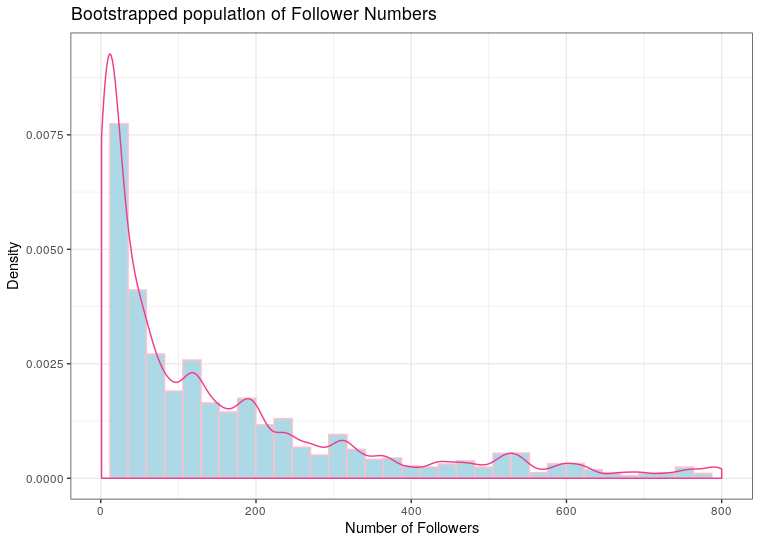
\includegraphics[width=12cm]{./Figures/BootStrap_Pop.png}
\caption{\label{fig:org1bcabb4}Histogram of the bootrapped population of follower counts}
\end{figure}

\subsubsection{b.) Estimate a Confidence Interval for Follower Counts}
\label{sec:org7374ef1}
\begin{itemize}
\item The normal \(t\) value bootstrap offers now advantage over using a \(t\) distribution (other than being illustrative of bootstrapping generally) \cite[Section 4.1]{hesterberg2015}
\item It is more appropriate to use a percentile interval for skewed data such as this, but it is still not very accurate \cite[Section 4.1]{hesterberg2015}

The \texttt{boot} package implements confidence intervals consistent with work by Davison and Hinkley \cite{ripley2020} in there texbook \emph{Bootstrap Methods and their Application} wherein the consensus is that \(BC_{a}\) methods will be  \cite[Ch. 5]{davison1997} superior to mere percentile methods in terms of accuracy. \cite[Ch. 5]{carpenter2000,davison1997}

Wait, hold on, the population is non-normal, sure, but the sampling distribution will obviously be normal, have I gotten confused?
\end{itemize}

\label{org3f0983d}
\bibliography{references}

\label{orgb8f0c16}
 \bibliographystyle{unsrt}
\end{document}
